\chapter{Resultados}

A equação do foguete, juntamente com os modelos e conceitos discutidos anteriormente, pode ser aplicada de forma prática para estudar diferentes configurações de veículos lançadores e suas capacidades de inserção de carga útil em órbita geossíncrona.

Com base nas aulas ministradas, é utilizado o veículo lançador brasileiro VLM-1 como ponto de partida, no qual podemos propor novos arranjos capazes de realizar diferentes missões de lançamento. O veículo lançador utiliza os motores S-44 e S-50, com seus dados de massa, de impulso específico e tração média. Esses dados são apresentados na Tabela \ref{tab:daods}.


\begin{table}[H]
\centering
\caption{Dados dos motores S-50 e S-44.} % Título da tabela
\label{tab:daods}
\begin{tabular}{@{}lllll@{}}
\toprule
Motor & $m_{p}[\mathrm{~kg}]$ & $m_{s}[\mathrm{~kg}]$ & $I_{s p}[\mathrm{~s}]$ & $\bar{F}[\mathrm{kN}]$ \\ \midrule
S-50  & 11058                 & 1367                  & 271                    & 440                    \\ 
S-44  & 813                   & 166,5                 & 270                    & 38                     \\ \bottomrule
\end{tabular}
\fonte{Notas de aula.} % Nota de rodapé
\end{table}

Também foi utilizado o motor RD-843, suas especificações podem ser vistas na Tabela \ref{tab:rdd}.

\begin{table}[H]
\centering
\caption{Dados do motor RD-843.} % Título da tabela
\label{tab:rdd}
\begin{tabular}{@{}ccccc@{}}
\toprule
Massa               & Tração             & Impulso específico & Número de queimas & Tempo de operação \\ \midrule
16,5 kg             & 2,5 kN             & 315,5 s            & 5                  & 700 s             \\ \bottomrule
\end{tabular}
\fonte{Notas de aula.} % Nota de rodapé
\end{table}

As configurações propostas são modificadas, alterando valores de parâmetros que serão exemplificados mais posteriormente.


Essa aplicação prática permitirá explorar e analisar diferentes configurações de veículos lançadores, considerando as restrições e requisitos específicos para alcançar uma órbita geossíncrona, e avaliar a viabilidade e desempenho desses sistemas para a realização da missão proposta.


%\begin{figure}[H]
%    \begin{center}
%        \caption{Coeficiente de arrasto contínuo em função do número de Mach}
%        \includegraphics[width=3.5in]{figuras/.png}
%        \label{fig:aerodin}
%       \fonte{(TEWARI,2007).}
%     \end{center}
%\end{figure}

\section{Impulso de Velocidade}

A primeira avaliação para a inserção orbital de um veículo lançador é realizada por meio do cálculo da capacidade de impulso de velocidade, $\Delta v$. Essa avaliação consiste em determinar a capacidade de $\Delta v$ de uma determinada configuração de veículo lançador para uma carga útil específica, conforme apresentado na seção \ref{sectionfoguete}.

No contexto da inserção em órbita geossíncrona, o requisito de $\Delta v$ necessário foi mencionado pelo professor durante a aula como $\Delta v_{req} = 13 km/s$. Esse valor representa o impulso total necessário para atingir a órbita geossíncrona, levando em consideração as perdas esperadas durante o lançamento, como a perda de arrasto.

Durante a avaliação, o valor de $\Delta v_{req}$ da configuração do veículo lançador é comparado com valores tabelados aproximados, levando em conta as perdas esperadas, a fim de determinar se a configuração proposta é capaz de atender ao requisito de $\Delta v_{req}$ para a inserção orbital geossíncrona.

Essa avaliação é crucial para garantir que o veículo lançador tenha a capacidade necessária para inserir a carga útil na órbita desejada e alcançar os objetivos da missão proposta.

Para a resolução desse parâmetro foi utilizado o código \textit{"estudo\_equacao\_foguete"}. O código é dividido em várias seções, começando com a definição de constantes, seguida dos dados das massas estruturais, massas de propelente e impulso específico ideal para cada configuração de foguete.

Em seguida, são realizados os cálculos, incluindo a determinação das razões estruturais, das massas totais no início da queima de cada estágio e das razões de carga útil para cada estágio e para a carga útil total. Esses cálculos são feitos para cada configuração de foguete.

A primeira simulação foi realizada com o três configurações apresentadas pelo professor em aula, C1, C2 e C3. OS dados de cada configuração podem ser vistos em \ref{tab:primeira}. Os dados já são apresentados considerando o acoplamento dos motores, considerando 550 kg de elementos de fixação no primeiro estágio e pequenas reduções no desempenho dos motores devido
às perturbações dos motores acoplados.

\begin{table}[H]
\centering
\caption{Dados das configurações de foguetes.}
\label{tab:primeira}
\begin{tabular}{ccccccc}
\toprule
Configuração & Estágio & Motores & $m_{p}[\mathrm{kg}]$ & $m_{s}[\mathrm{kg}]$ & $I_{s p}[\mathrm{s}]$ & $F[\mathrm{kN}]$ \\
\midrule
C-1 & 1 & $3 \times S-50$ & 33157 & 4650 & 251 & 1317 \\
 & 2 & $1 \times S-50$ & 11058 & 1367 & 271 & 455 \\
 & 3 & $1 \times S-44$ & 813 & 166,5 & 270 & 33 \\
\midrule
C-2 & 1 & $3 \times S-50$ & 33157 & 4650 & 251 & 1317 \\
 & 2 & $1 \times S-50$ & 11058 & 1367 & 271 & 455 \\
 & 3 & $1 \times R D-843$ & 609 & 161,9 & 315 & 2,5 \\
\midrule
C-3 & 1 & $3 \times S-50$ & 33157 & 4650 & 251 & 1317 \\
 & 2 & $1 \times S-50$ & 11058 & 1367 & 271 & 455 \\
 & 3 & $4 \times R D-843$ & 811 & 228,7 & 315 & 10 \\
\bottomrule
\end{tabular}

\fonte{Notas de aula.}
\end{table}

A partir do códigos, temos na Tabela \ref{tab:primeirosdados}, os resultados para essas configurações. Observa-se que para todos os casos o $\Delta v < \Delta v_{req}$, fazendo com que a escolha de configuração seja rejeitada.

\begin{table}[H]
\centering
\caption{Valores de $\Delta v$ para as configurações C-1, C-2 e C-3.}
\label{tab:primeirosdados}
\begin{tabular}{cccc}
\toprule
Configuração & C-1 & C-2 & C-3 \\
\midrule
$\Delta v[\mathrm{km} / \mathrm{s}]$ & 11,712 & 12,041 & 11,669 \\
\bottomrule
\end{tabular}

\fonte{Autores.}
\end{table}

Após isso foram feitas outras simulações, alterando os parâmetros da a configuração 2, a qual foi que a gerou resultados mais precisos na primeira simulação. Foi feito uma varredura utilizando o código \textit{"estudo\_foguete\_otimizado"}, no qual foram comparados os desempenhos de utilizar 3xS50, 4xS50, 5xS50 ou 7xS50 no primeiro estágio, e variando a massa de propelente do 3 estágio. 

Os resultados para essa simulação podem ser vistos na Figura \ref{fig:motores}, e nela é possível ver que a configuração de foguete com 7 motores S50 atinge a maior mudança de velocidade ($\Delta v$) quando a massa de propelente do terceiro estágio é aumentada em cerca de $37\%$. Nesse ponto, temos que $\Delta v = 13,34 km/s$, o que satisfaz o pré requisito.

\begin{figure}[H]
    \begin{center}
        \caption{Variação do $\Delta v$ para diferentes configurações}
        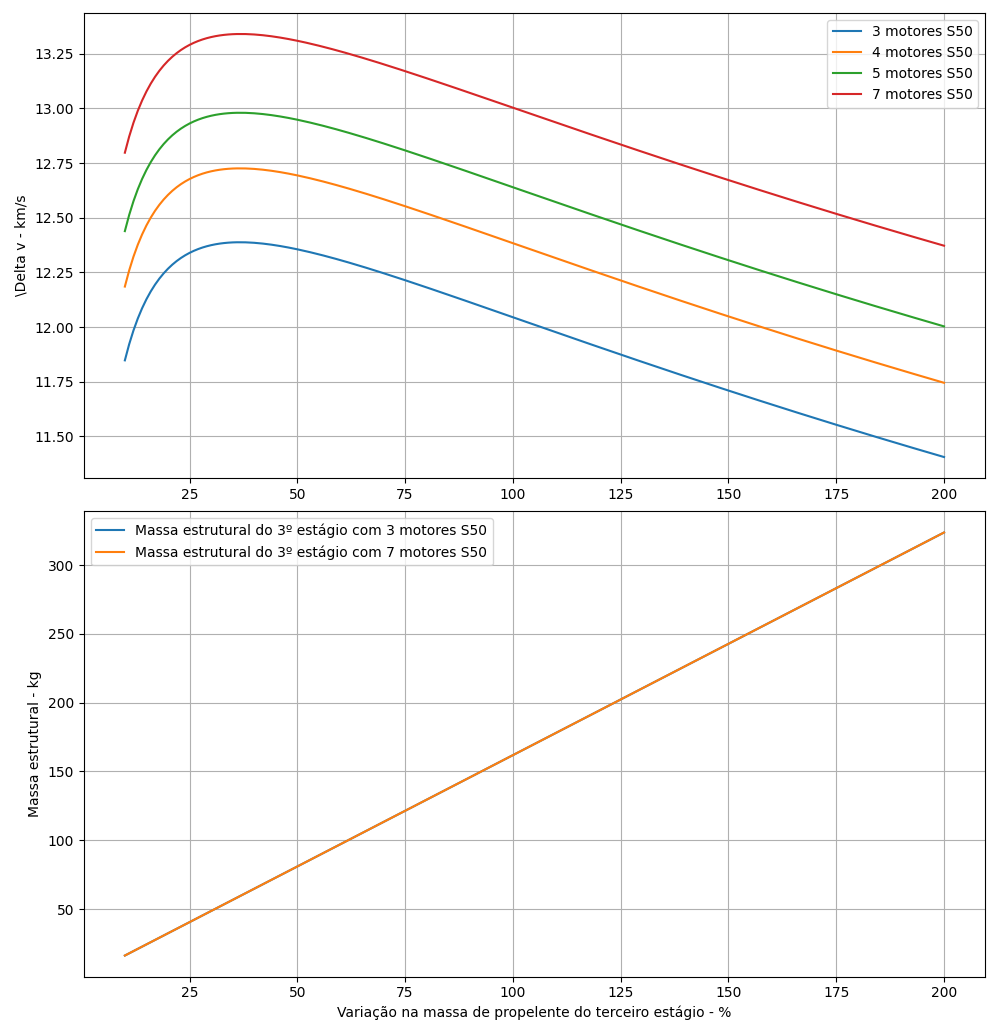
\includegraphics[width=4.5in]{figuras/motores.png}
        \label{fig:motores}
      \fonte{Autores.}
     \end{center}
\end{figure}

Portanto, a configuração final do foguete pode ser vista na Tabala \ref{tab:final}.

\begin{table}[h]
\centering
\caption{Configuração Final} 
\label{tab:final}
\begin{tabular}{cccccc}
\hline
Estágio & Motores & $m_{p}[\mathrm{~kg}]$ & $m_{s}[\mathrm{~kg}]$ & $I_{s p}[\mathrm{~s}]$ & $F[\mathrm{kN}]$ \\
\hline
1 & $7 \times S-50$ & 77366 & 7750 & 251 & 3073 \\
2 & $1 \times S-50$ & 11058 & 1367 & 271 & 455 \\
3 & $1 \times R D-843$ & 225.33 & 64.75 & 315 & 2.5 \\
\hline
\end{tabular}

\fonte {Autores.}
\end{table}

\section{Energia Específica}

A configuração, uma vez testada pela primeira vez, é submetida à análise de viabilidade com relação à energia específica. No contexto do caso em discussão, o objetivo é atingir uma órbita geossíncrona (GSO - Geosynchronous orbit), identificada por uma velocidade orbital de $n_{\text{gso}} = 7.2921 \times 10^{-5} \text{rad/s}$ e semieixo maior $a_{\text{gso}}= 42.164 \times 10^{6} \text{m}$ (6.61 vezes o raio da Terra).

Para a realização da verificação, escolhemos uma órbita circular de referência com raio $r_{\text{ref}} = a_{\text{gso}} = 42.164 \times 10^{6} \text{m}$, correspondente a uma altitude $h_{\text{ref}} = 35.785863 \times 10^{6} \text{m}$. Se a energia específica, no instante da inserção na órbita, exceder esse valor, tal órbita é alcançável por tal veículo, necessitando apenas de uma modificação das condições quando o motor do terceiro estágio for desligado.

A inspeção do voo de sondagem é realizada de maneira eficaz com base na velocidade relativa e na posição no referencial rotativo PCPF.Para isso foram utilizados os códigos que dizem respeito as dinâmicas do foguete, e os principais resultados podem ser vistos na Figura \ref{fig:sondagem}. 

Os dados utilizados para rodar o programa \textit{"voo\_sondagem\_3\_estagios"} foram os mesmo fornecidos como output do código \textit{"estudo\_foguete\_otimizado"}, sendo eles:

\begin{table}[h]
\centering
\caption{Dados para rodar o voo de sondagem} 
\label{tab:final}
\begin{tabular}{cccccc}
\hline
Estágio & Motores & $m_{p}[\mathrm{~kg}]$ & Tempo de queima [s]\\
\hline
1 & $S-50$ & 77366 &  62 \\
2 & $S-50$ & 11058 & 62 \\
3 & $R D-843$ & 225.33 & 278.43 \\
\hline
\end{tabular}

\fonte {Autores.}
\end{table}

\begin{figure}[H]
    \begin{center}
        \caption{Voo de sondagem.}
        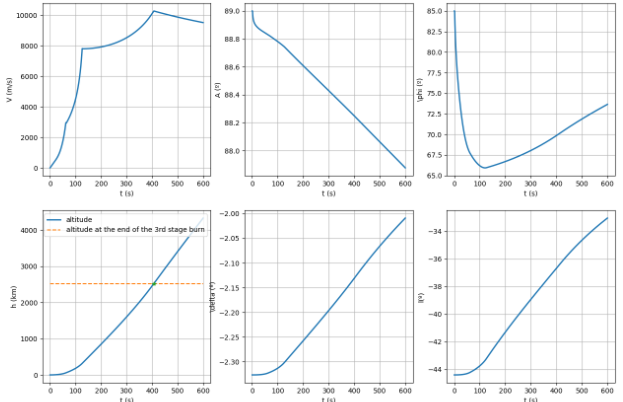
\includegraphics[width=6in]{figuras/voosondagema.png}
        \label{fig:sondagem}
      \fonte{Autores.}
     \end{center}
\end{figure}
\newpage


Porém, para estudar a inserção na órbita, é necessário calcular a velocidade inercial e a posição no referencial inercial ICP, a partir das quais os parâmetros orbitais podem ser avaliados. Então esses resultados são convertidos e podem ser vistos na Figura \ref{fig:parametrossondagem}.

\begin{figure}[H]
    \begin{center}
        \caption{Parâmetros inerciais do voo de sondagem.}
        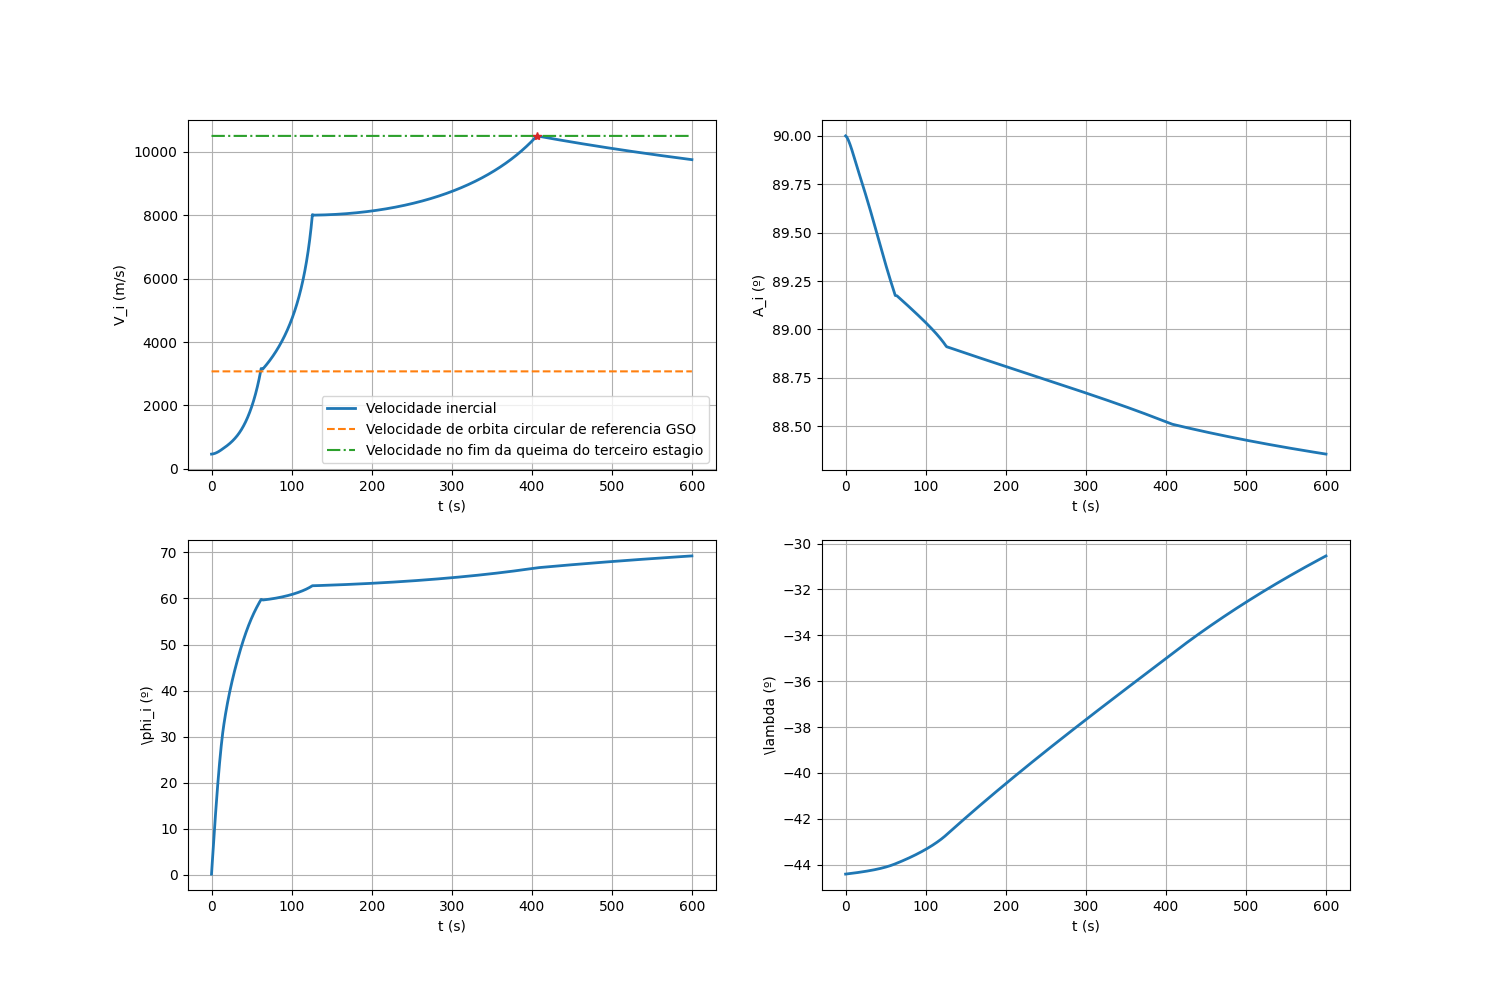
\includegraphics[width=7in]{figuras/parametrossondagem.png}
        \label{fig:parametrossondagem}
      \fonte{Autores.}
     \end{center}
\end{figure}

\newpage

Os parâmetros inerciais, incluindo a velocidade inercial e a posição no referencial inercial, são fundamentais para a determinação dos parâmetros orbitais. Ao utilizar código como o \textit{"det\_orbita"}, é possível computar estes parâmetros orbitais. Além disso, o código \textit{"calcula\_auxiliares"} é utilizado para calcular a energia específica do voo de sondagem. Os resultados podem ser vistos na Figura \ref{fig:energiaespecificasondagem}.


\begin{figure}[H]
    \begin{center}
        \caption{Energia específica e parâmetros orbitais.}
        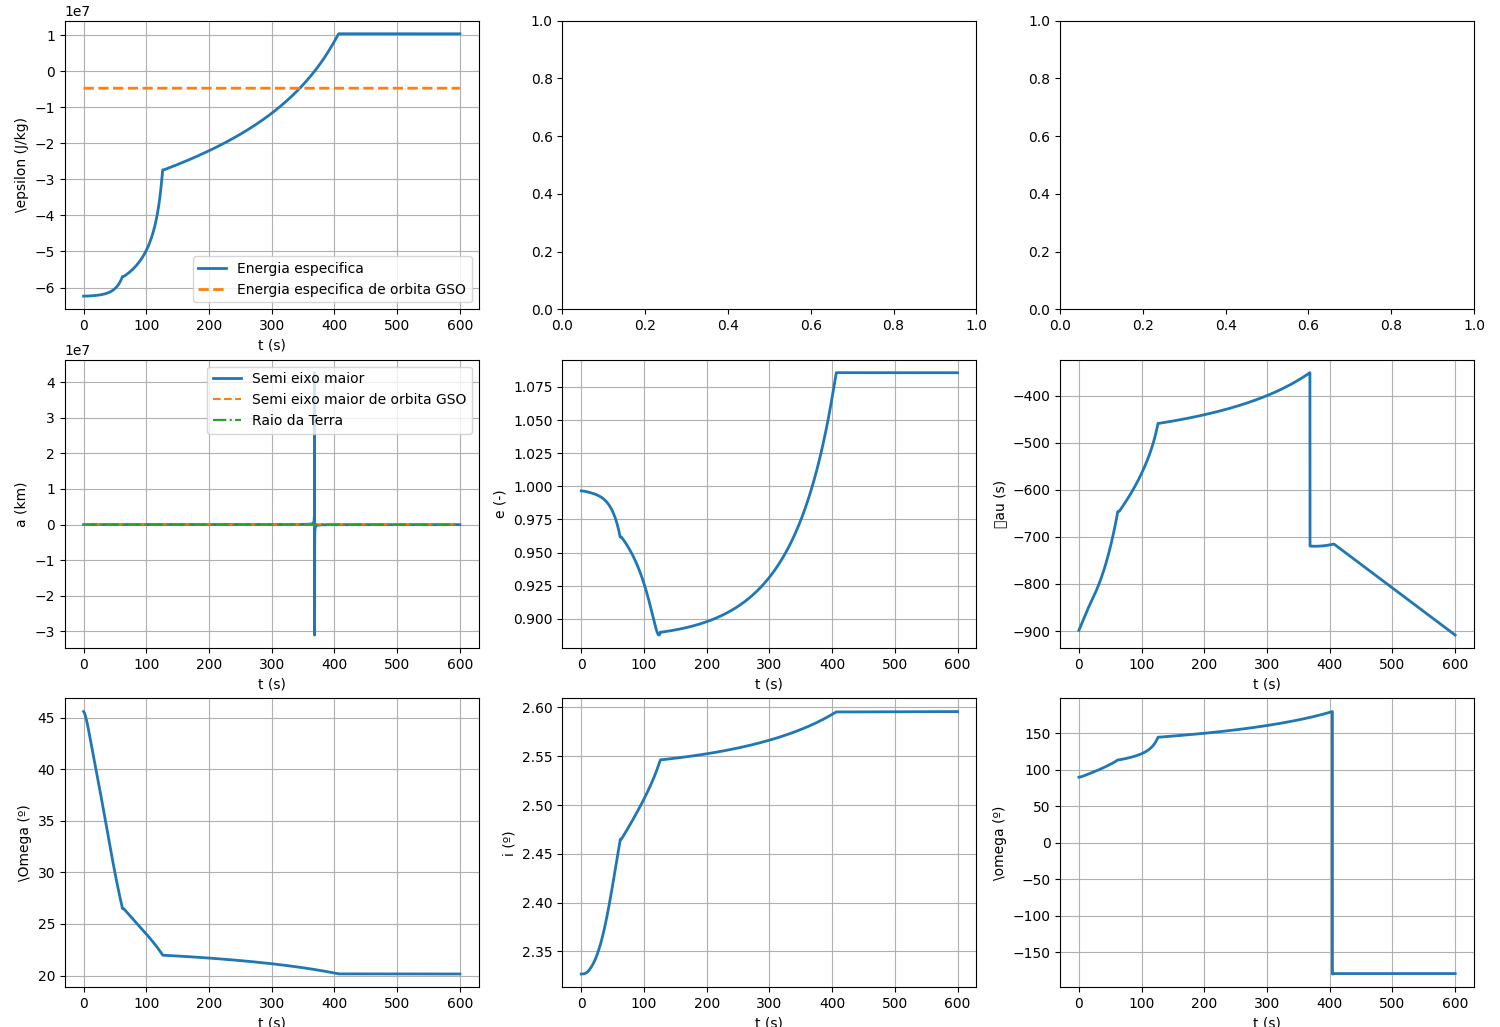
\includegraphics[width=5.8in]{figuras/energiaespecificasondagem.png}
        \label{fig:energiaespecificasondagem}
      \fonte{Autores.}
     \end{center}
\end{figure}

A interpretação mais importante dessa figura é a de no primeiro gráfico, a linha pontilhada representa a energia de referência necessária para atingir a órbita do problema, e a azul é a energia específica do foguete. Percebe-se que no momento que ocorre a inserção orbital, o foguete possui energia suficiente para tal.

Na Figura \ref{fig:3} podemos observar os tempos de queima de cada estágio, sendo os dois estágios iniciais com maior tempo de queima e maior empuxo gerado, enquanto o terceiro estágio possui uma única queima, rápida e com baixo empuxo gerado, que praticamente não pode ser observado sem zoom na imagem. Além disso, é possível notar a diminuição de massa após a massa ser ejetada durante a queima. 

\begin{figure}[H]
    \begin{center}
        \caption{Tempo de queima dos estágios.}
        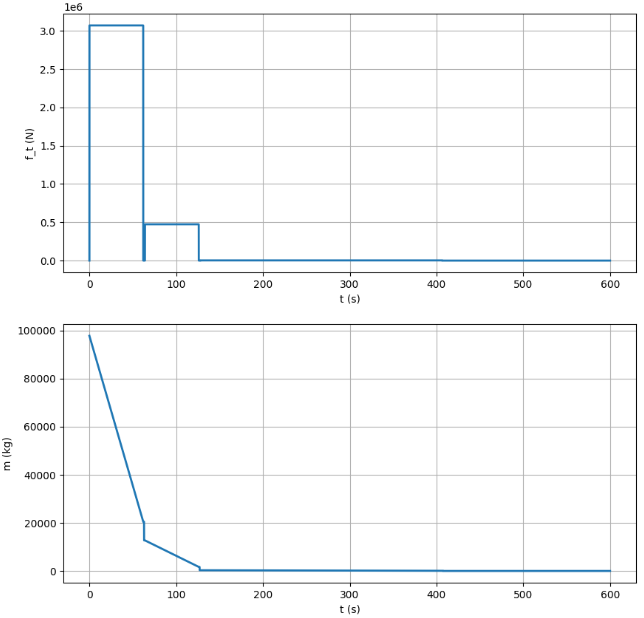
\includegraphics[width=3.4in]{figuras/fig3aula27.png}
        \label{fig:3}
      \fonte{Autores.}
     \end{center}
\end{figure}

Já na Figura \ref{fig:4} são plotados os resultados referentes as condições atmosféricas. Durante o lançamento, o arrasto, a densidade do ar e também a pressão dinâmica são maiores nos primeiros instantes, enquanto a temperatura tende a aumentar ao longo do lançamento. O número de Mach sofre grandes variações até aproximadamente três minutos após o lançamento, quando tende a se estabilizar.

\begin{figure}[H]
    \begin{center}
        \caption{Condições atmosféricas.}
        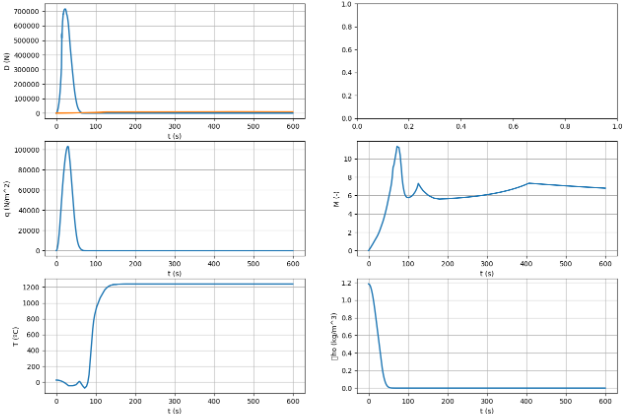
\includegraphics[width=4.5in]{figuras/fig4aula27a.png}
        \label{fig:4}
      \fonte{Autores.}
     \end{center}
\end{figure}

\section{Inserção em órbita GSO}
%%%%%%%% AULA 28%%%%%%%5
Para viabilizar a órbita GSO, é necessário utilizar do reacendimento do motor, que é a capacidade de um foguete ligar novamente, ou reacender, seus motores após eles terem sido desligados inicialmente. No caso do trabalho, isso é dado por múltiplas ignições do motor do último estágio, que é ignitado duas vezes. No caso, a primeira ignição coloca o foguete em órbita baixa com periastro numa altitude suficiente para sofrer baixo arrasto atmosférico, podendo essa ser uma órbita circular (estacionamento) ou excêntrica (transferência). Como a órbita utilizada é a de transferência, é necessário controlar o tempo de queima do último estágio em termos da elevação inercial da velocidade. Quando o ângulo de trajetória da velocidade inercial for zero, é necessário desligar o motor do último estágio, sendo esse o perigeu da órbita de transferência. Nesse momento, a velocidade inercial deve ser compatível com a velocidade de perigeu da órbita de transferência cujo apogeu é igual ao raio da órbita desejada, que é a órbita geossíncrona. 

Os dados de tempo de queima utilizados para a simulação foram:

\begin{table}[h]
\centering
\caption{Tempos de ignição e queima.}
\begin{tabular}{|c|c|}
\hline
\textbf{Descrição} & \textbf{Tempo (s)} \\
\hline
Tempo de Ignição & 580 \\
\hline
Tempo de Queima 1 & 213 \\
\hline
Tempo de Queima 2 & 66 \\
\hline
\end{tabular}

\fonte {Autores.}
\end{table}


Após adaptar os códigos e inserir os valores definidos, são gerados os outputs mostrados nas tabelas a seguir.

\begin{table}[H]
\centering
\caption{Parâmetros do foguete}
\begin{tabular}{|l|l|}
\hline
\textbf{Parâmetro} & \textbf{Valor} \\
\hline
Área ref. com 1o estágio ($m^2$) & 7.666666666666667 \\
Área ref. com 2o estágio ($m^2$) & 1.2345485272815064 \\
Área ref. com 3o estágio ($m^2$) & 0.977426364075326 \\
Área ref. da carga útil ($m^2$) & 0.786214389183969 \\
Massa ini. ant. queim. do 1o estágio (kg) & 97844.0844 \\
Massa ini. ant. queim. do 2o estágio (kg) & 12728.0844 \\
Massa ini. ant. queim. do 3o estágio (kg) & 303.0844 \\
Massa da carga útil (kg) & 13 \\
Razões estruturais & [0.09105221 0.11002012 0.22322607] \\
Razões de carga útil & [0.13008537 0.02381226 0.04289234] \\
Velocidades de exaustão (m/s) & [2461.46915 2657.60215 3089.09475] \\
Razão de carga útil total & 0.00013286444530314395 \\
Impulso de velocidade total ideal (m/s) & 13449.786837505853 \\
Cond. fin. de azimute de vel. inercial (grau) & 85.5731667395659 \\
Cond. ini. de azimute de vel. relativa (grau) & 85.35329334311488 \\
\hline
\end{tabular}

\fonte {Autores.}
\end{table}

\begin{table}[H]
\centering
\caption{Órbita GSO requerida}
\begin{tabular}{|l|l|}
\hline
\textbf{Parâmetro} & \textbf{Valor} \\
\hline
Raio da órbita GSO (km) & 42164.14 \\
Velocidade da órbita GSO (km/s) & 3.0746611796284924 \\
\hline
\end{tabular}

\fonte {Autores.}
\end{table}

\begin{table}[H]
\centering
\caption{Parâmetros da Órbita Obtida}
\begin{tabular}{|l|l|}
\hline
\textbf{Parâmetro} & \textbf{Valor} \\
\hline
Velocidade no momento da inserção orbital (km/s) & 7.915448092085045 \\
Altitude no momento da inserção orbital (km) & 3718.864788180722 \\
Distância radial no momento da inserção orbital (km) & 10097.001788180722 \\
Semi eixo maior (km) & 24454.165121965787 \\
Período (min) & 168.28615193314312 \\
Raio do perigeu (km) & 5474.673352743322 \\
Raio do apogeu (km) & 43433.65689118826 \\
Altitude do perigeu (km) & -903.463647256678 \\
Altitude do apogeu (km) & 37055.519891188254 \\
\hline
\end{tabular}

\fonte {Autores.}
\end{table}

\begin{table}[H]
\centering
\caption{Parâmetros da Órbita GTO Requerida}
\begin{tabular}{|l|l|}
\hline
\textbf{Parâmetro} & \textbf{Valor} \\
\hline
Perigeu da órbita GTO requerida (km) & 5474.673352743322 \\
Apogeu da órbita GTO requerida (km) & 42164.14 \\
Semi eixo maior da órbita GTO requerida (km) & 23819.406676371662 \\
Velocidade de perigeu da órbita GTO requerida (km/s) & 11.352615669084885 \\
Velocidade de apogeu da órbita GTO requerida (km/s) & 1.4740455393487284 \\
T disparo do propulsor do 3o estágio após a separação do 2º (s) & 580 \\
Duração do 1o disparo do motor do 3o estágio (s) & 215 \\
Duração do 2o disparo do motor do 3o estágio (s) & 64 \\
Momento do 2o disparo do motor do 3o estágio (s) & 18687.654012214116 \\
Impulso de vel. requerido para circ. da órbita (km/s) & 1.600615640279764 \\
Massa prop. requerida para circ. da órbita (kg) & 52.345023780248965 \\
Massa prop. disp. para o 3o disparo (kg) & 51.68860215053763 \\
\hline
\end{tabular}

\fonte {Autores.}
\end{table}

\begin{table}[H]
\centering
\caption{Parâmetros da Órbita Final}
\begin{tabular}{|l|l|}
\hline
\textbf{Parâmetro} & \textbf{Valor} \\
\hline
Período (min) & 1467.496828363403 \\
Semi eixo maior (km) & 42777128.41405425 \\
Excentricidade & 0.014695116017340595 \\
Inclinação (º) & 4.928454244752832 \\
\hline
\end{tabular}

\fonte {Autores.}
\end{table}

Além dos outputs gerados que foram mostrados nas tabelas anteriores, também são gerados os gráficos com as variáveis ao longo do lançamento e os gráficos de trajetória do veículo. 

\begin{figure}[H]
    \begin{center}
        \caption{Variáveis inerciais da órbita final.}
        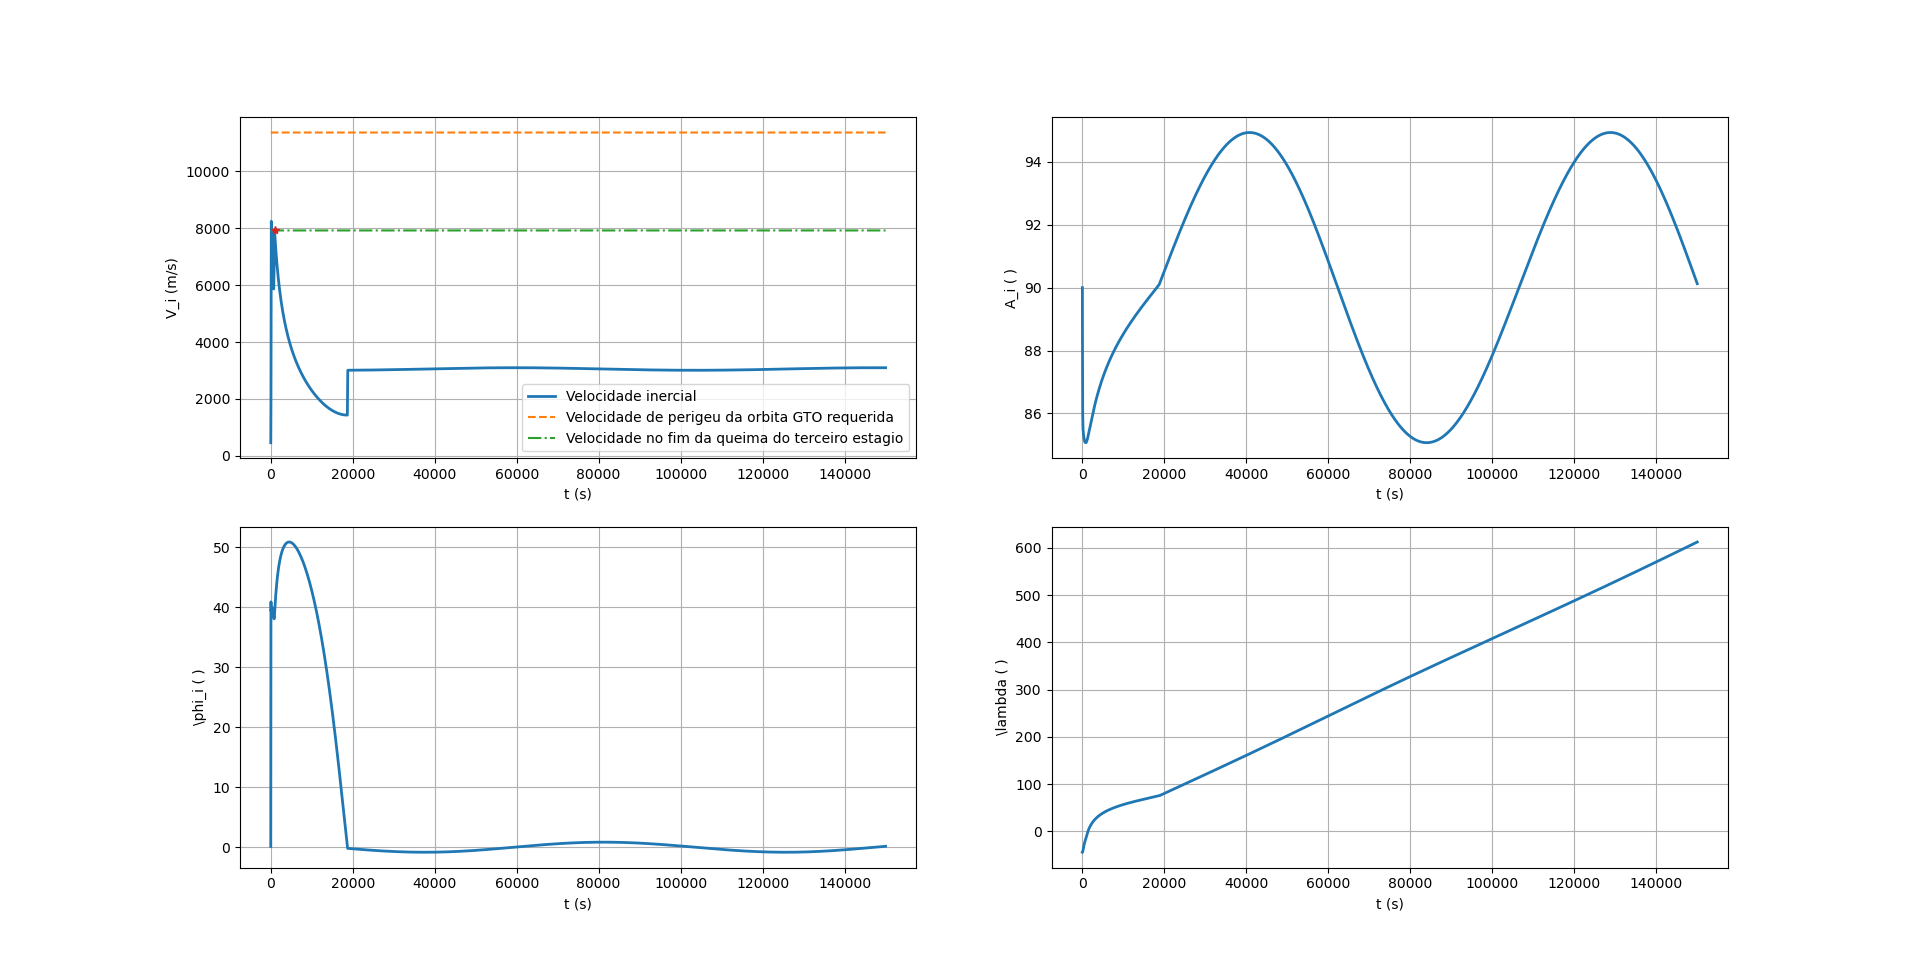
\includegraphics[width=6in]{figuras/Figure_2.png}
        \label{fig:3}
      \fonte{Autores.}
     \end{center}
\end{figure}

É interessante notar que a velocidade de perigeu da órbita GTO requerida não foi atingida, porém a velocidade foi suficiente para a inserção em órbita GSO. Além disso, o ângulo do Azimute varia muito durante o lançamento. 

\begin{figure}[H]
    \begin{center}
        \caption{Variáveis atmosféricas.}
        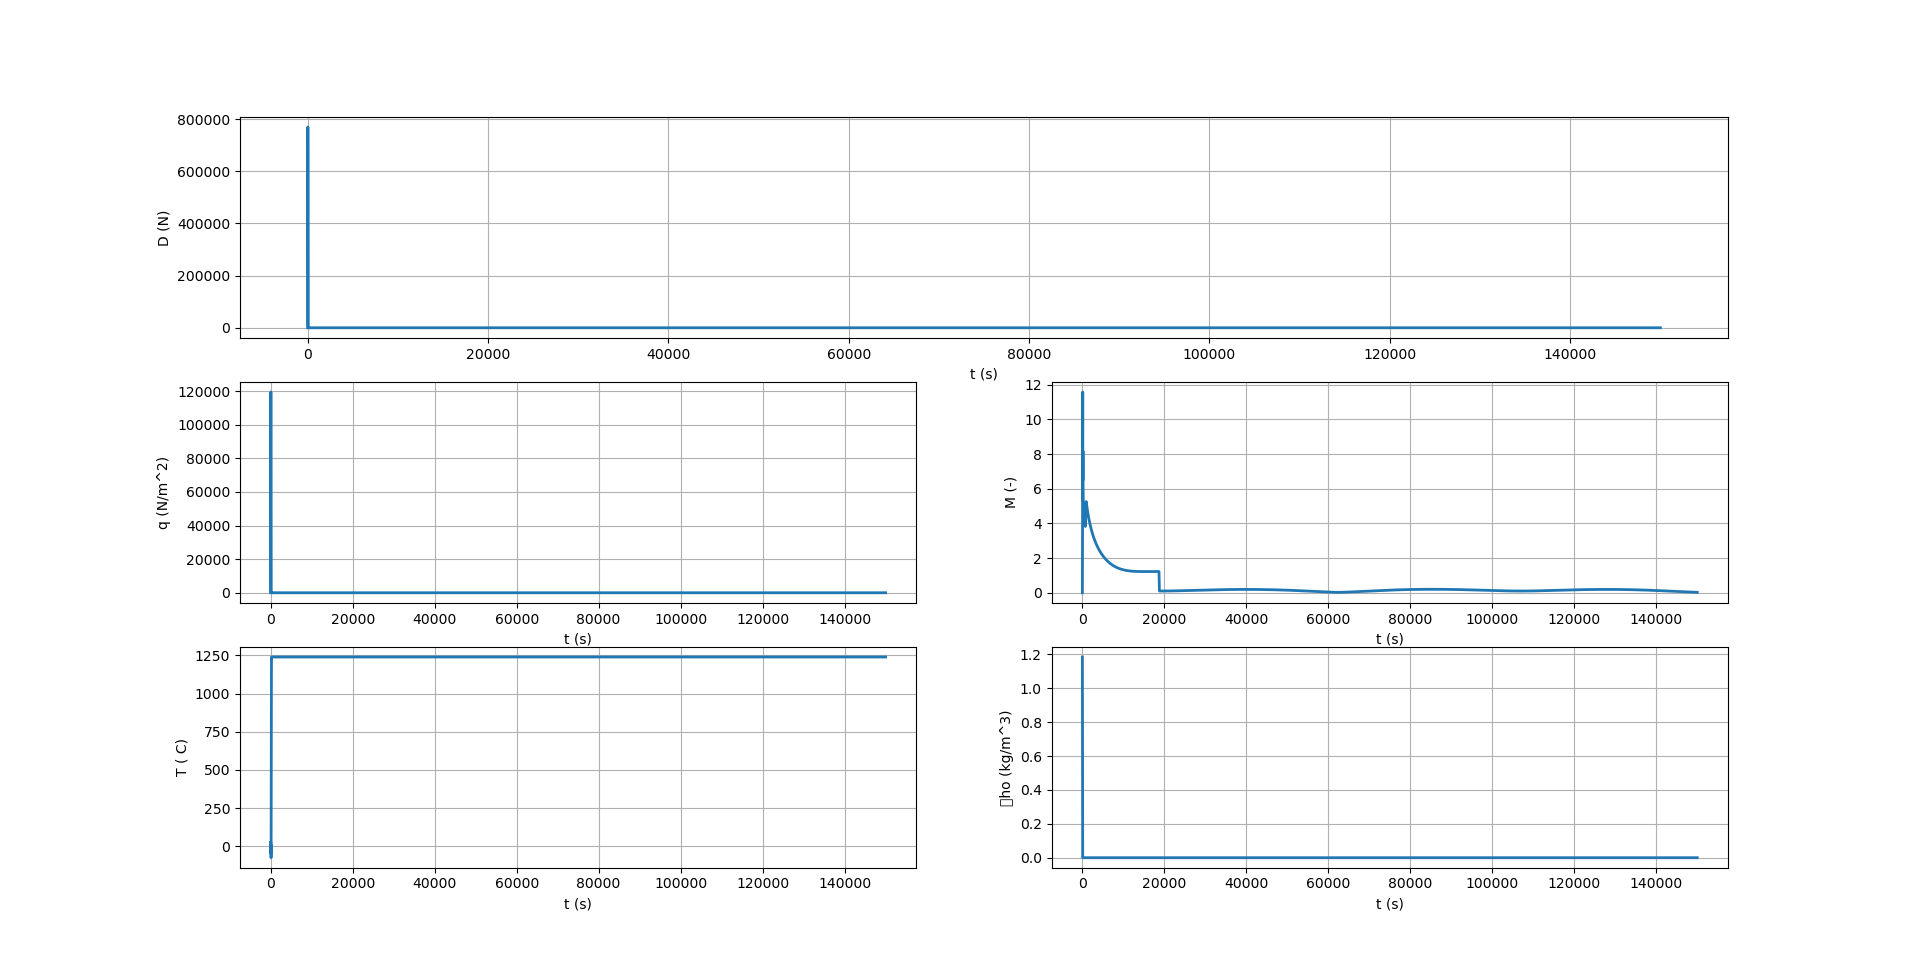
\includegraphics[width=6in]{figuras/Figure_4.png}
        \label{fig:3}
      \fonte{Autores.}
     \end{center}
\end{figure}

Como dito anteriormente, as variáveis atmosféricas influenciam principalmente durante os primeiros instantes do lançamento, após isso, conforma a altitude aumenta, esses feitos tendem a diminuir e influenciar pouco. Além disso, para a inserção em órbita GSO, é necessário levar o foguete até um pouco em que o mesmo sofra com baixas forças atmosféricas.

\begin{figure}[H]
    \begin{center}
        \caption{Parâmetros da órbita final.}
        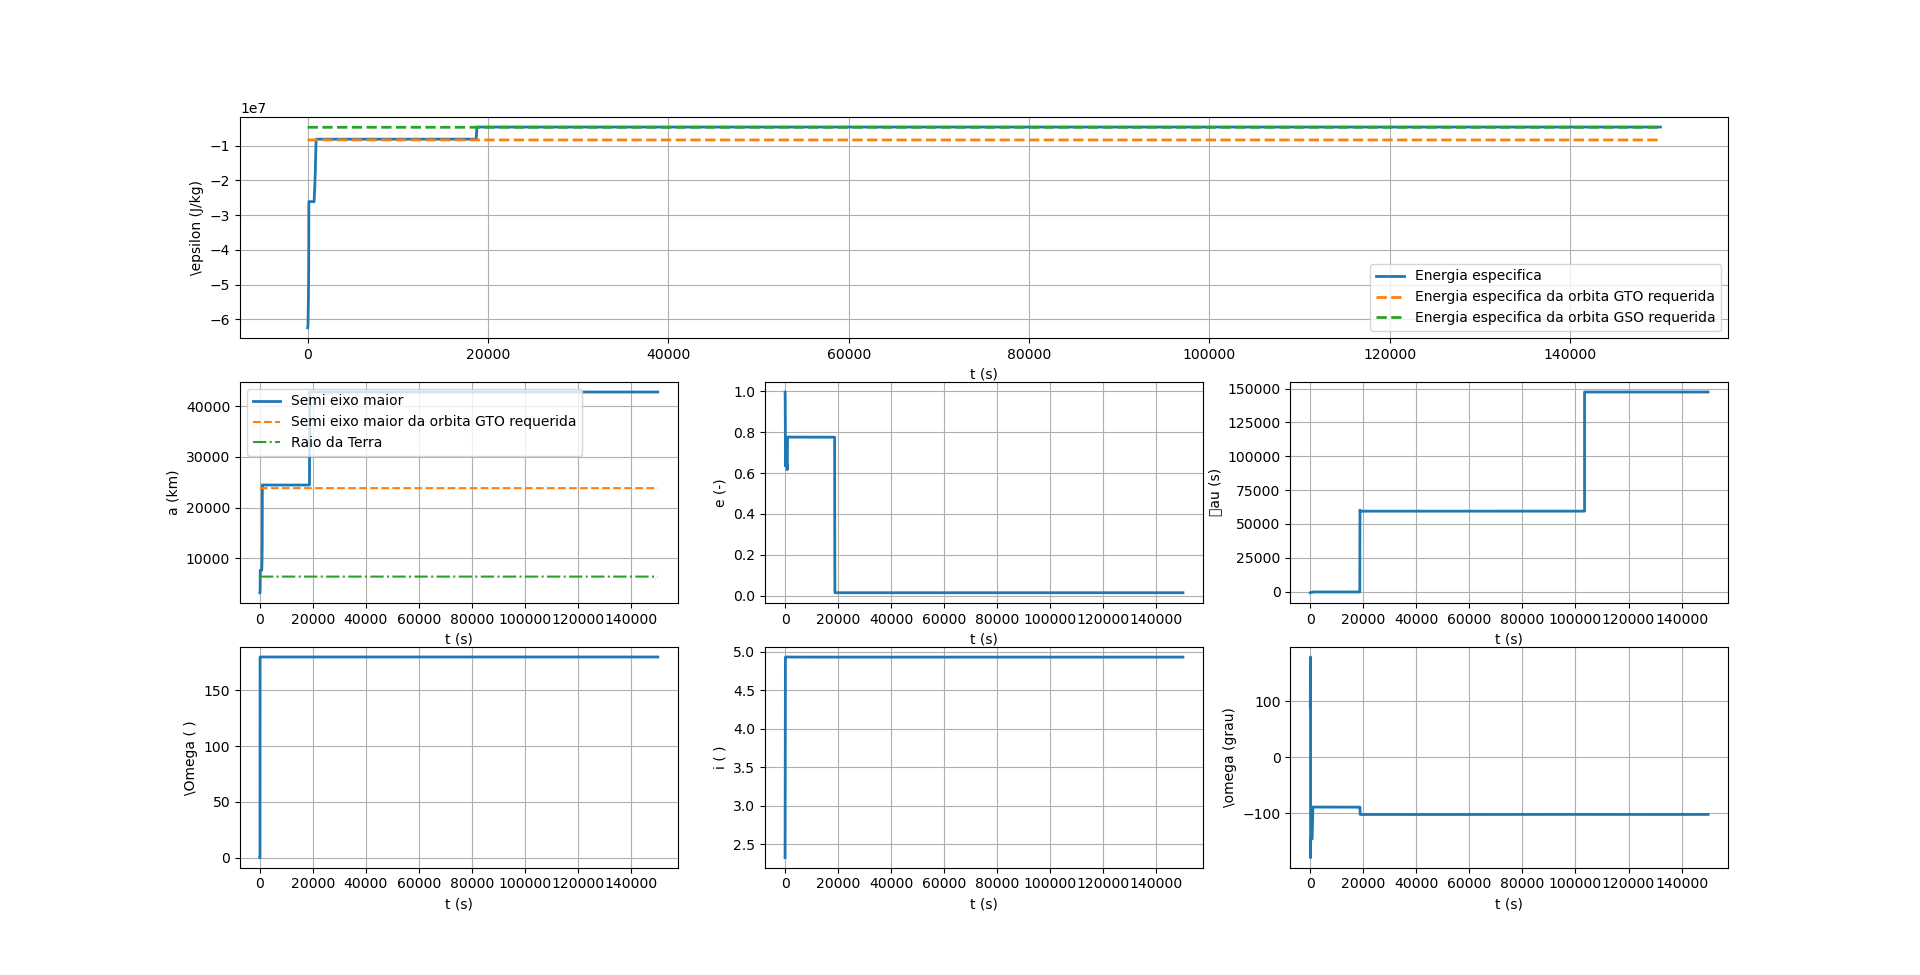
\includegraphics[width=6in]{figuras/Figure_5.png}
        \label{fig:3}
      \fonte{Autores.}
     \end{center}
\end{figure}

A energia específica para a órbita geossíncrona foi atingida após a energia específica para a órbita GTO ser atingida, resultando no sucesso da inserção na órbita GSO utilizando múltiplas ignições do motor do último estágio, que foi ignitado duas vezes.

\begin{figure}[H]
    \begin{center}
        \caption{Variáveis durante o lançamento.}
        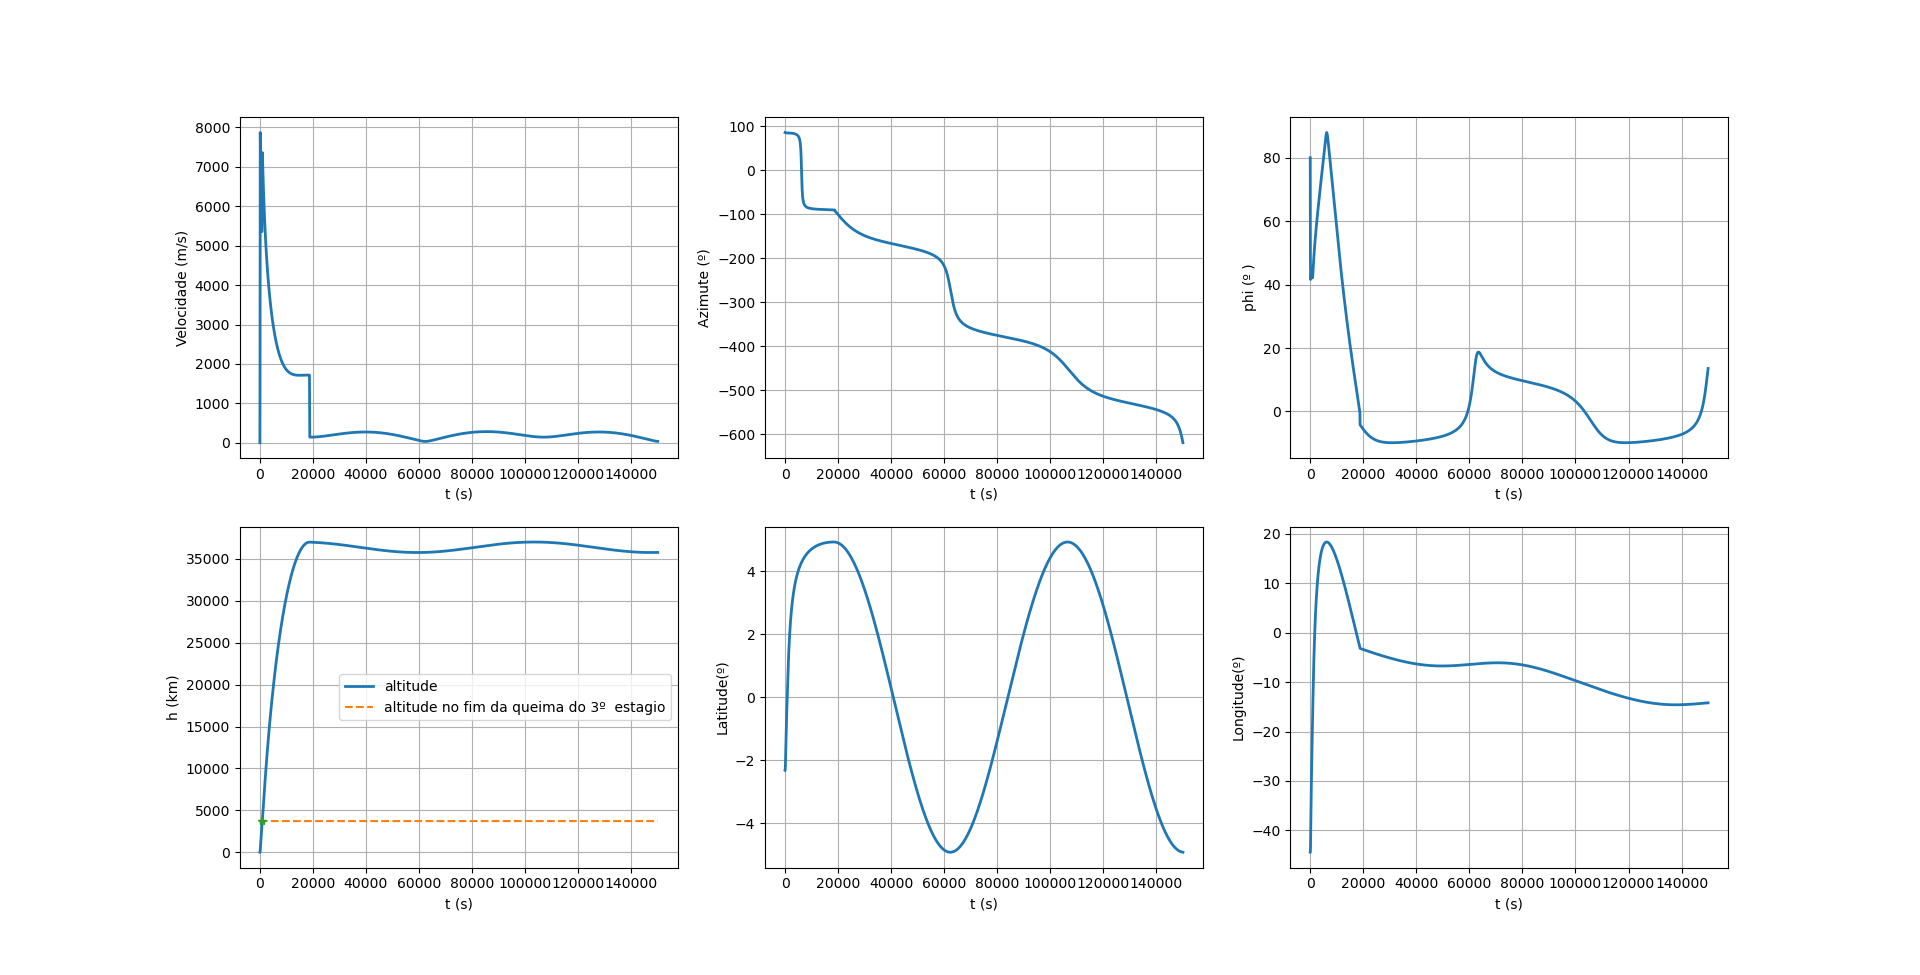
\includegraphics[width=6in]{figuras/Figure_1.png}
        \label{fig:3}
      \fonte{Autores.}
     \end{center}
\end{figure}

A altitude continua aumentando após o fim da queima do terceiro estágio e passa a se estabilizar após a segunda queima do terceiro estágio. A velocidade tem seu pico logo no início do lançamento, sofrendo variação durante a queima do segundo estágio e, por fim, pequenas variações ao longo das queimas do terceiro estágio. Novamente, o Azimute sofre grandes variações, junto da elevação. 

\begin{figure}[H]
    \begin{center}
        \caption{Órbita final atingida pelo veículo.}
        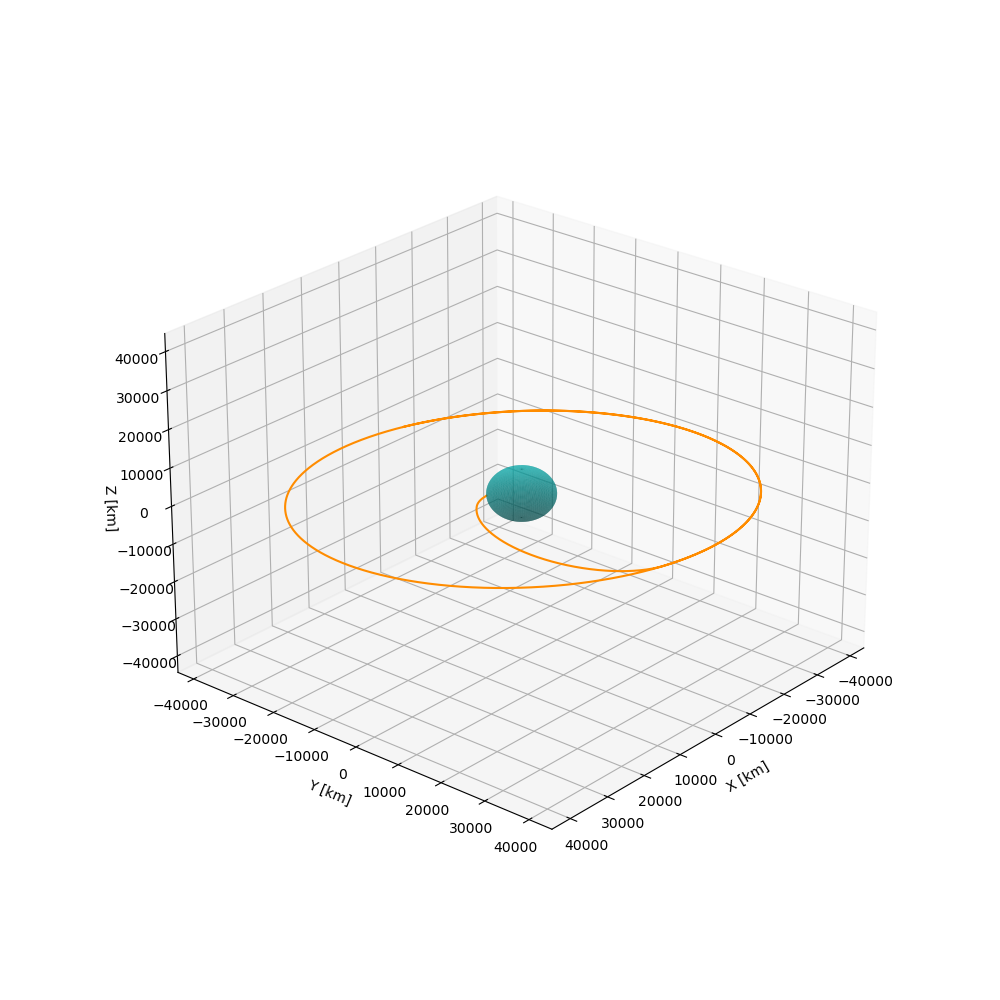
\includegraphics[width=6in]{figuras/fig_6.png}
        \label{fig:3}
      \fonte{Autores.}
     \end{center}
\end{figure}

É possível notar que a órbita geossíncrona foi atingida utilizando os dados descritos anteriormente utilizando praticamente toda a massa de propelente disponível. É visto que a excentricidade é quase nula, sendo um requisito para órbitas geossíncronas. 

\par No gráficos gráficos abaixo, fica claro que a maior energia é utilizada durante os primeiros minutos da missão, sendo essa necessária para "vencer" a força do campo gravitacional terrestre e o arrasto atmosférico. Isso é percebido pelo picos de força propulsiva e do arrasto. 
\begin{figure}[H]
    \begin{center}
        \caption{Valores atingidos durante a queima.}
        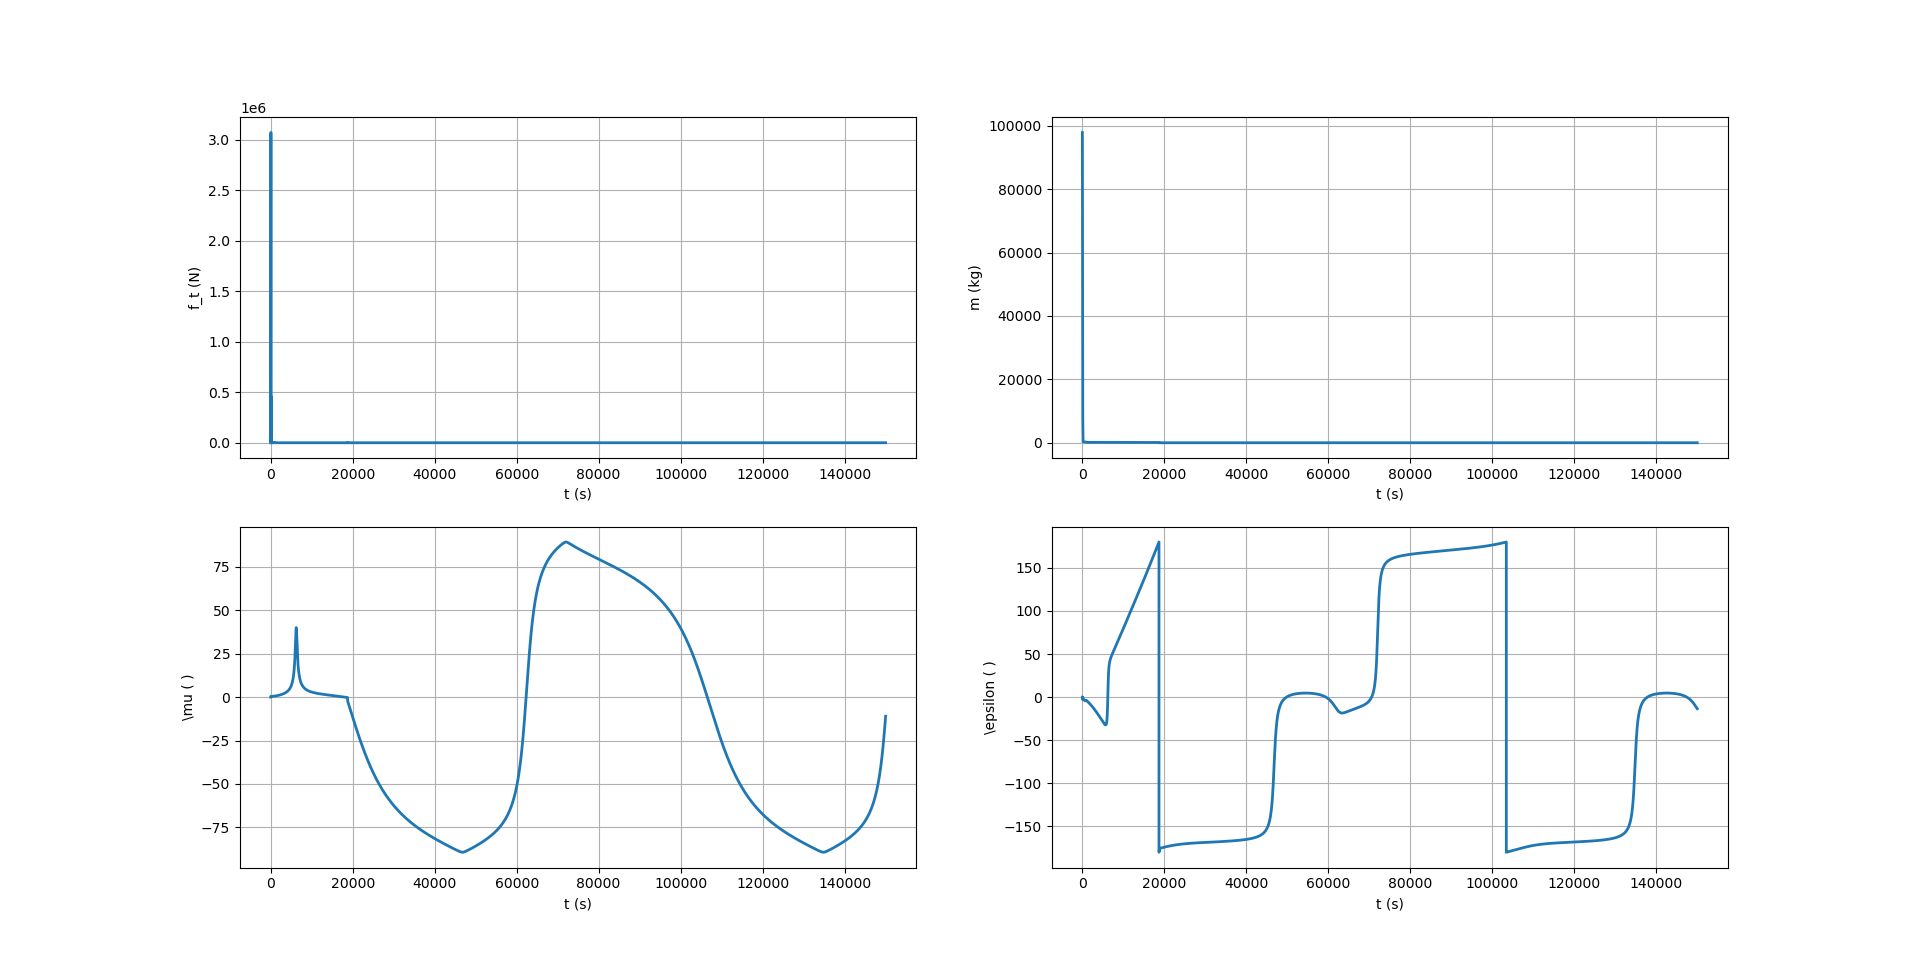
\includegraphics[width=6in]{figuras/Figure_3.png}
        \label{fig:3}
      \fonte{Autores.}
     \end{center}
\end{figure}


\chapter{Conclusão}
\input{Texto/Conclusão}
\chapter{Trabalhos futuros}

Pesquisas futuras poderiam concentrar-se na modulação da direção dos foguetes, especificamente no controle do apontamento do bocal propulsor. Uma estratégia promissora seria o desenvolvimento de um algoritmo de controle inovador, cuja eficácia seria avaliada sob uma variedade de condições de voo. Adicionalmente, a análise do controle das superfícies de empenagem de foguetes poderia desempenhar um papel crucial na otimização da dinâmica de voo. Tal investigação tem o potencial de incrementar a estabilidade e a eficiência do voo do foguete, contribuindo para avanços significativos nesta área. Para uma avaliação mais fidedigna do comportamento dos foguetes em voo, sugere-se a utilização de dados oriundos de lançamentos reais, ao invés da aplicação exclusiva de estimativas teóricas. Essa metodologia ofereceria uma visão mais autêntica do desempenho do foguete em condições reais de voo. Outra linha de investigação poderia contemplar a alteração do design do foguete e a distribuição de massa no seu interior. Isso poderia incluir a modificação da forma do foguete ou a reconsideração da quantidade e disposição do combustível. Essas mudanças poderiam levar a melhorias significativas no desempenho dos foguetes.